\section{Proposed Methodology}
The SmartGrid Sentinel framework operates as a decoupled sequence forecasting pipeline, visualized in Fig. 1.

\begin{figure}[htbp]
\centering
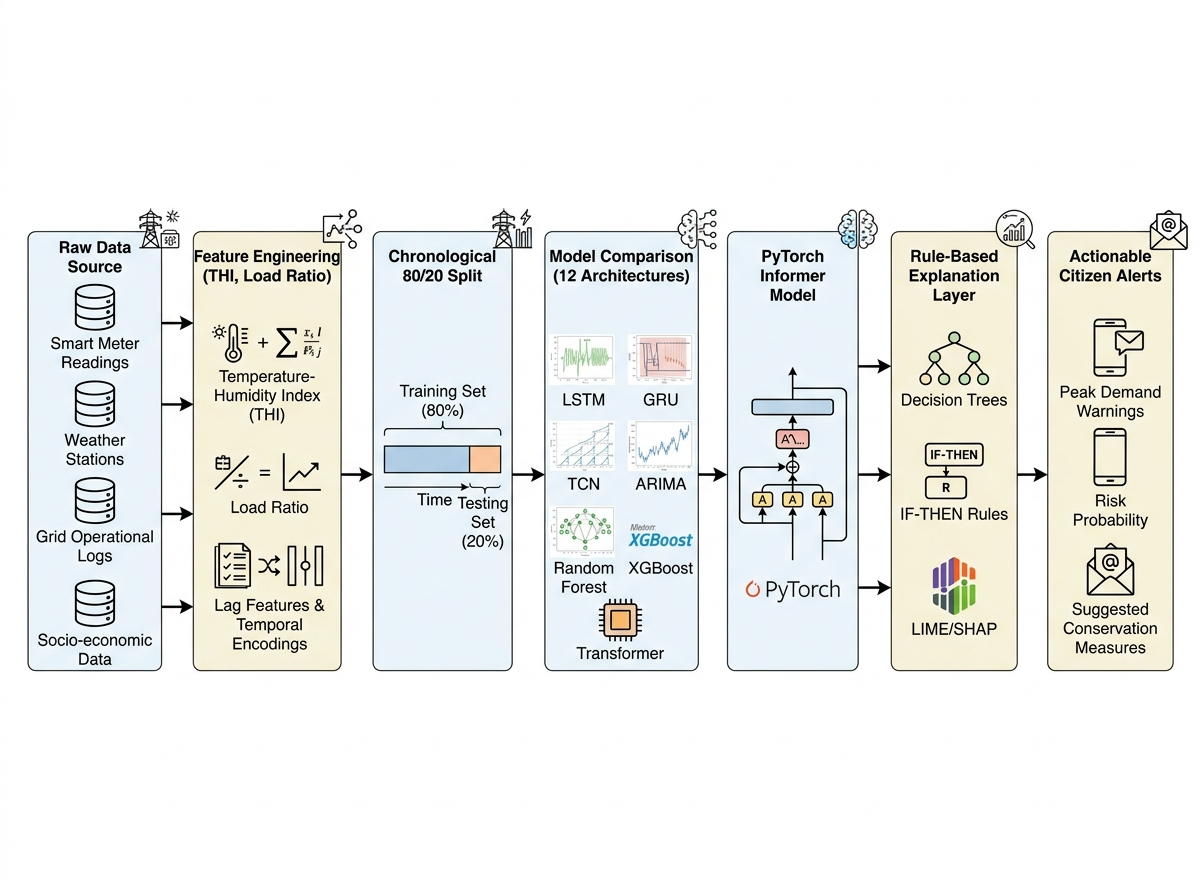
\includegraphics[width=\linewidth]{fig1.jpg}
\caption{System Architecture of SmartGrid Sentinel.}
\label{fig:arch}
\end{figure}

The primary forecasting component is the Informer model. It uses multi-head self-attention mechanisms to map historical features $X_{t-4:t}$ to future risk labels $y_{t+1}$. The Informer structure utilizes self-attention blocks combined with feed-forward neural layers, concluding with a Softmax output projecting the probability distribution of three risk classes: Low, Medium, and High.

The rule-based explainability layer sits on top of the model output. If the model predicts a Medium or High risk level, this module executes deterministic rules based on the input telemetry to output textual explanations (e.g., matching overload bounds or high THI values) without claiming direct visualization of deep feature attribution.
